\chapter[Results and Discussion]{Results and Discussion}
In this section we will review the main results of the thesis. Their significance and relation to 
other works in the literature will be discussed.

\section[Force Fields Development]{Force Field Development}\label{ffdevelopment}
\subsection[Actinyl Force Fields In Solution]{Actinyl Force Fields In Solution}
The largest body of force fields designed concerned the actinyl cations. In particular 
\ce{[AnO2*(H2O)5]^{2+}} for An=U, Np, Pu, Am and \ce{[NpO2*(H2O)5]^{+}}. This work was 
rooted in a chapter of the thesis of F. Torrico, a former PhD student of the group\cite{thesisFran}.

These are the first hydrated ion models for actinyls and 
the first to have a molecular cation rather than a monoatomic cation. Using an interaction 
potential which contains the \textit{ab initio} information of the system is very convenient in 
actinoid systems. Unlike other compounds, the lack of experimental data complicates parametrizing
actinoid compounds empirically\cite{Ions_in_sol_and_Marcus_2016}. 

\begin{figure}
\centering 
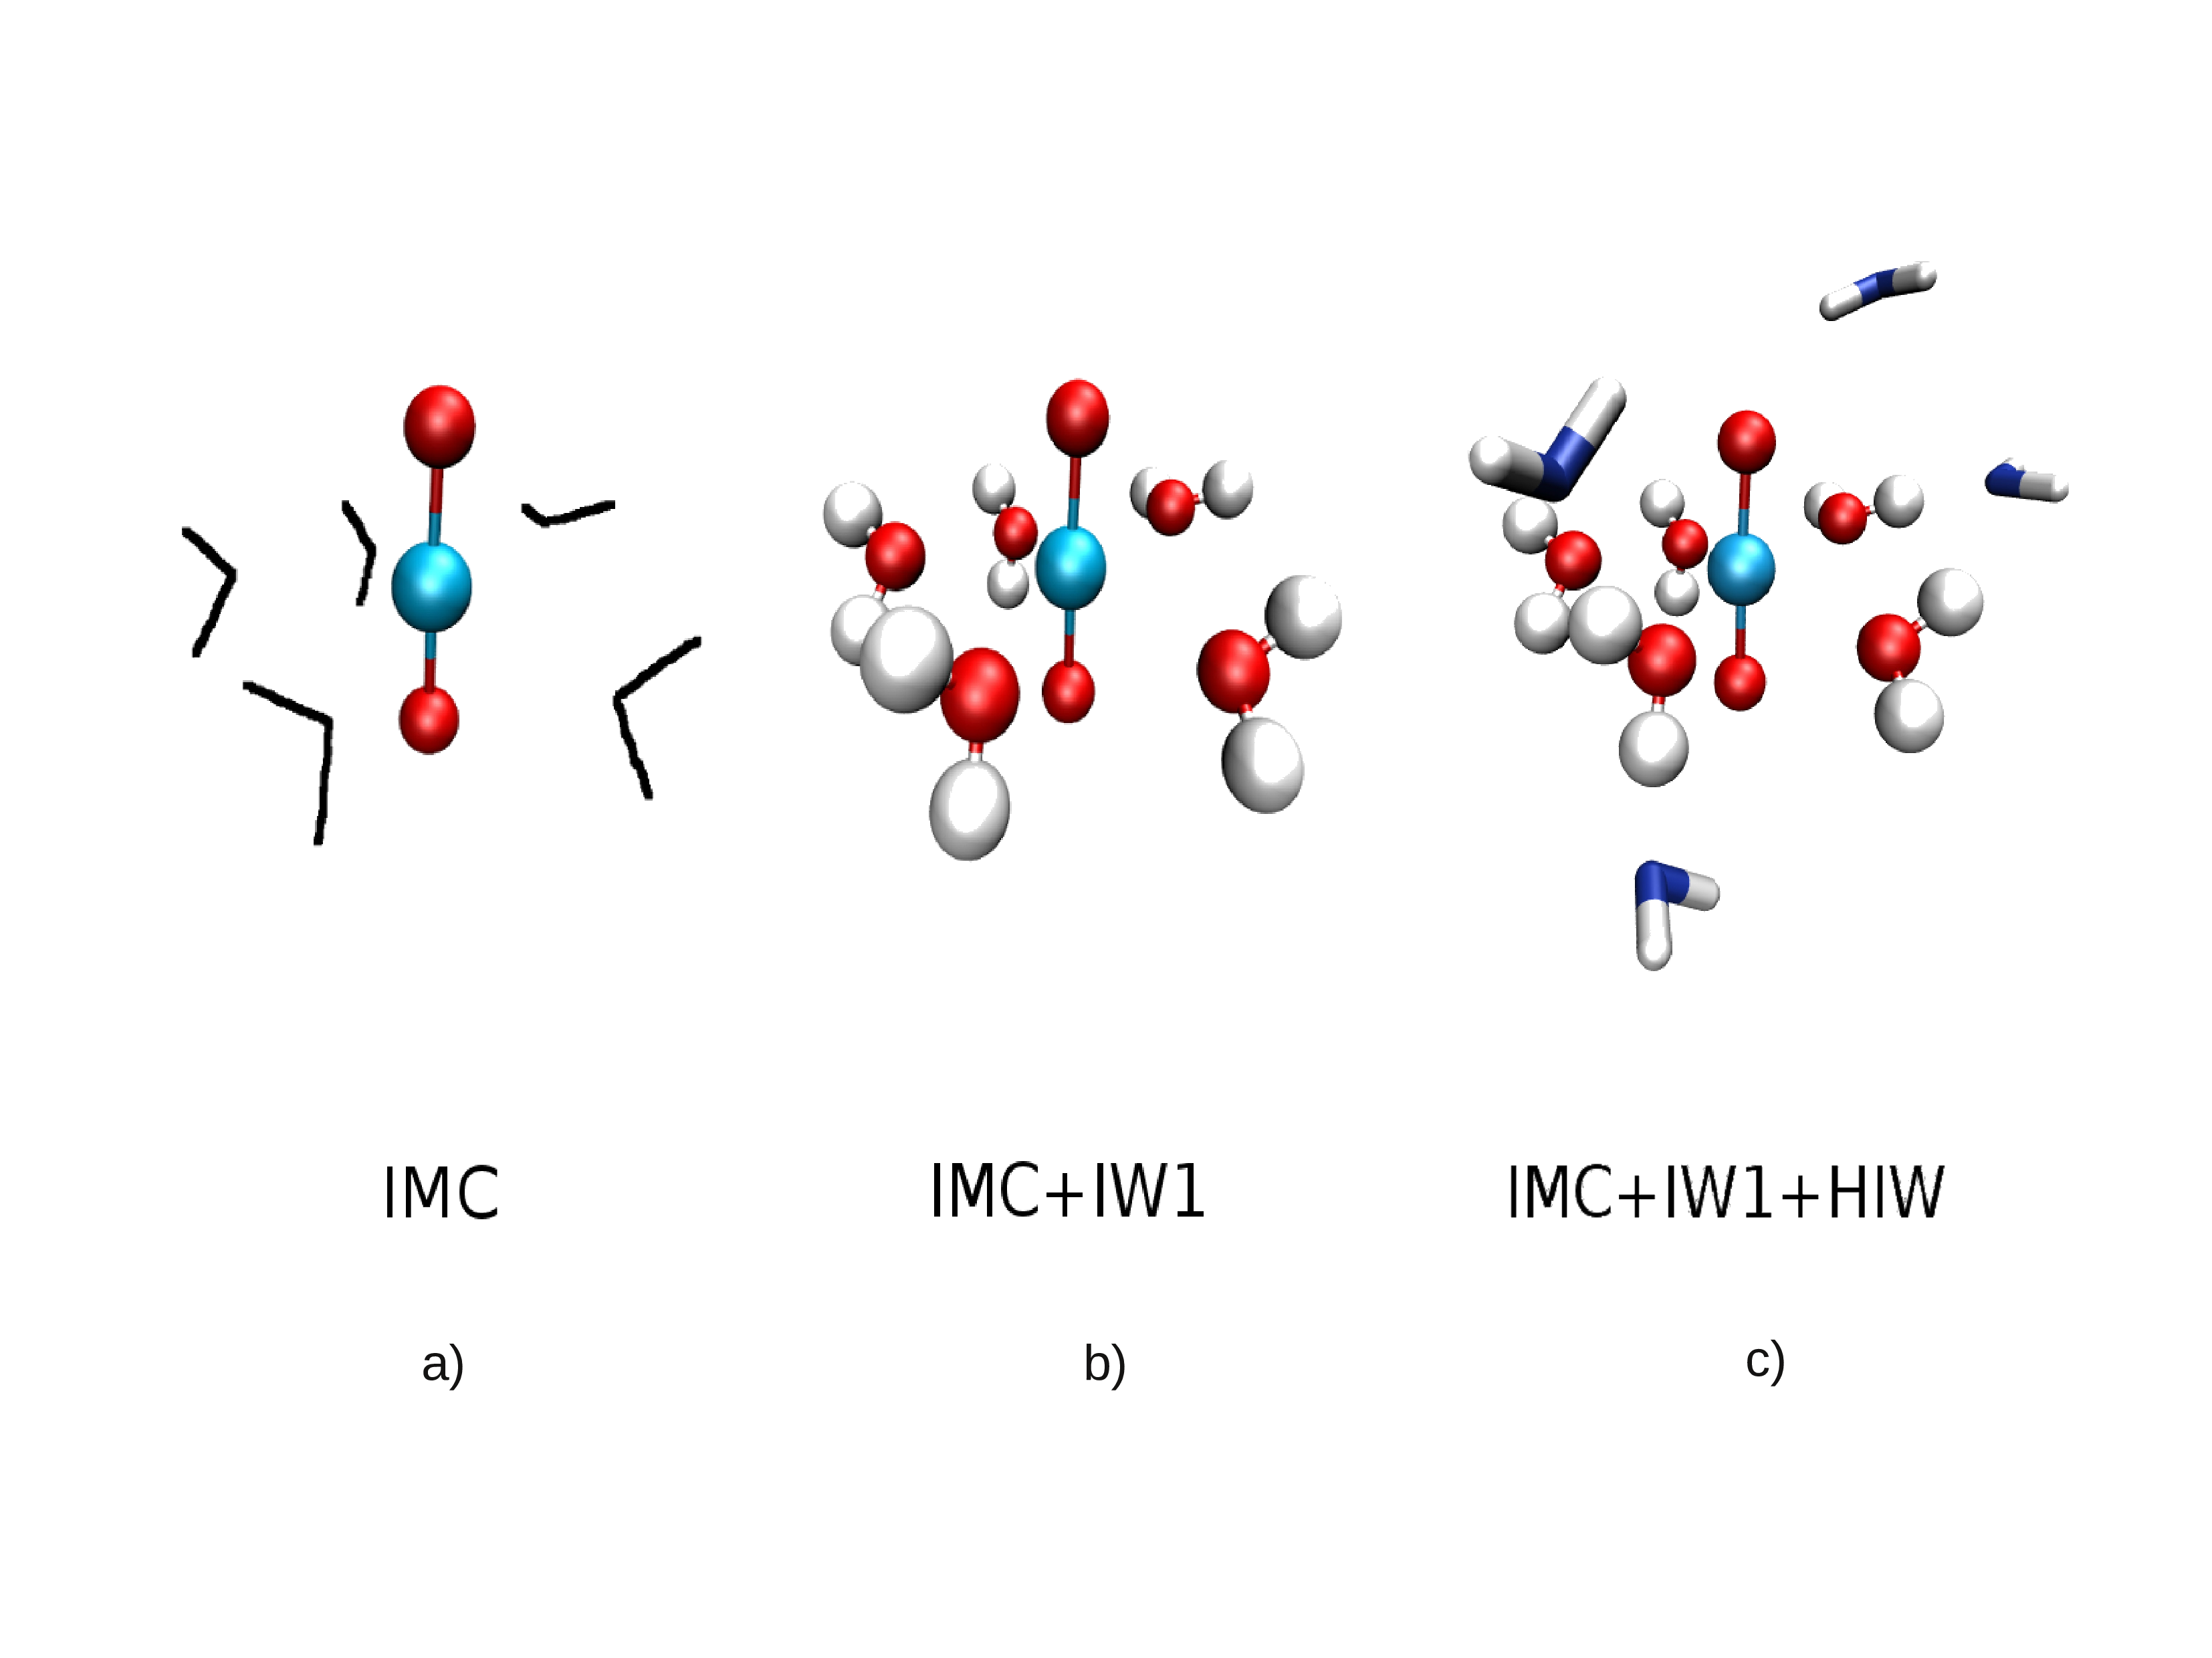
\includegraphics[width=10cm]{./images/IMCIW1HIW.png}
\caption[Components of the Hydrated Ion Model]{Schematic representation of the components of 
the HIM force field of actinyl ions. The 
ball and stick representation shows the atoms involved in each of the terms. In a) the first shell 
is not fully 
drawn since it does not participate in the IMC but they are added to calculate the interaction 
energies for the IMC following the HIM. }\label{HIM_actinyl}
\end{figure}

The actinyl force fields were developed using as reference structure the pentahydrate 
cation, 
\ce{[AnO2*(H2O)5]^{2+/+}}. The interaction potential was split into four components:
\begin{equation}
E=E_\text{IMC}+E_\text{IW1}+E_\text{HIW}+E_\text{W-W}
\end{equation}
The first three components are shown in Figure \ref{HIM_actinyl}. The 
first interaction 
potential is the Intra-Molecular Cation (\gls{imc}). This interaction potential controls the motion 
within the molecular cation, \ce{[AnO2]^{2+/+}}. It has the following mathematical expression:
\begin{equation}\label{eq1}
E_{\text{IMC}} = \sum_{i}^{ \substack{\text{O}_{\text{yl}} \vspace{0.02cm}\\ \text{sites} } }\left(
\frac{C_{4}^{\text{AnO}_{\text{yl}   }} }  {r_{\text{AnO}_{\text{yl,i}}}^{4} }  +
\frac{C_{6}^{\text{AnO}_{\text{yl}   }} }  {r_{\text{AnO}_{\text{yl,i}}}^{6} }  +
\frac{C_{8}^{\text{AnO}_{\text{yl}   }} }  {r_{\text{AnO}_{\text{yl,i}}}^{8} }  \right. \left.+
\frac{C_{12}^{\text{AnO}_{\text{yl}   }} }  {r_{\text{AnO}_{\text{yl,i}}}^{12} }\right)  +
\sum_{i}^{\substack{\text{O}_{\text{yl}} \vspace{0.02cm}\\ 
\text{sites} }}
\frac {q_{\text{An}} q_{\text{O}_{\text{yl,i}}}} { r_{\text{AnO}_{\text{yl,i}}} }
\end{equation}
The second term (Equation \ref{eq2}) is the ion-first shell water interaction (\gls{iw1}). In our model 
we have assumed that the first-shell
water molecules to be rigid and have the geometry of the gas phase optimization of the 
hydrated 
ion. 
The IW1 term makes the aqua ion flexible. It has the following mathematical expression:
\begin{equation}\label{eq2}
E_{\text{IW1}} = \sum_{i}^{ \substack{\text{AnO}_{\text 2} \vspace{0.02cm}\\ \text{sites} }}
  \frac {C_{4}^{\text{iO}_{\text I}}}{r_{\text{iO}_{\text I}}^{4}}
+ \frac {C_{6}^{\text{iO}_{\text I}}}{r_{\text{iO}_{\text I}}^{6}}
+ \frac {C_{8}^{\text{iO}_{\text I}}}{r_{\text{iO}_{\text I}}^{8}} 
+ \frac {C_{12}^{\text{iO}_{\text I}}}{r_{\text{iO}_{\text I}}^{12}} 
+ \sum_{i}^{ \substack{\text{AnO}_{\text 2} \vspace{0.02cm}\\ \text{sites} }}\,
\sum_{j}^{ \substack{\text{1}^{\text {st}}\text{ shell water}\vspace{0.02cm}\\ \text{sites} }}
\frac{q_{\text{i}}q_{\text{j}}}{r_{\text{ij}}}\\
\end{equation}
The final term (Equation \ref{eq3}) is the hydrated ion-bulk water interaction potential (\gls{hiw}). 
This term parametrizes 
the
interaction of the hydrated ion with any of the bulk water molecules (second shell and further). It 
has the 
following mathematical expression:
\begin{equation}\label{eq3}
E_{\text{HIW}} = \sum_{i}^{\substack{\text{HI} \vspace{0.02cm}\\ \text{sites} }} 
\sum_{j}^{\substack{\text{water} \vspace{0.02cm}\\ \text{sites} } }\left(
\frac{C_{4}^{ij}}{r_{ij}^{4}}+\frac{C_{6}^{ij}}{r_{ij}^{6}}+\frac{C_{8}^{ij}}{r_{ij}^{8}}\right.+
\frac{C_{12}^{ij}}{r_{ij}^{12}} +
\left.\frac{q_{i}q_{j}}{r_{ij}}\right)
\end{equation}
The employed bulk water model was TIP4P\cite{TIP4P_JChemPhys_Jorgensen_1983}. 

The partial charges appearing in Equations \ref{eq1}-\ref{eq3} were assigned with the 
Merzt-Kollmann 
method\cite{MK1_Kollman_JCompChem_1984,MK2_MerzKollman_JCompChem_1990}. These charges were 
calculated in the gas pha\-se QM minimum energy structures and using a wavefunction 
polarized by bulk solvent represented by a Polarizable Continuum Model (\gls{pcm} 
)\cite{PCM1_ChemPhys_Tomasi_1981,PCM2_JChemPhys_Tomasi_1997}. In 
the case 
of \ce{[NpO2*(H2O)5]^{+}} only the actinyl unit was given partial charges. Due to the low charge 
transfer and polarization of this monocation, the first-shell geometries and charges were taken to 
be 
equal to those of the TIP4P water model. The coefficients of the 
force fields were parametrized with a series of QM scans. $E_\text{IMC}$ and 
$E_\text{IW1}$ were parametrized with deformations following the main normal modes of the 
pentahydrate: symmetric and asymmetric An-\ce{O_{yl}} tension, \ce{O_{yl}}-An-\ce{O_{yl}} bending 
and lengthening of a An-\ce{O_{W1}} distance. $E_\text{HIW}$ was parametrized with scans of a 
second-shell water molecule moving around the hydrated ion at different distances and orientations. 
The root mean square errors of the fits were about 1-\SI{3}{\kcalmol}. All the interaction 
potentials 
were 
calculated specifically for every cation except for the HIW potential which was proven to be very 
similar across the cations studied. The level of theory for the quantum chemistry calculations was 
B3LYP with Stuttgard semi-relativistic pseudopotentials and their recommended basis sets on 
actinoids and aug-PVDZ on light 
atoms\cite{B3LYP1,B3LYP2_GAUSSIAN,DunningBasisSet3_Dunning_JChemPhys_1993,RECPStuttgart}. In all 
electronic structure calculations the first shell of water molecules was included. This was done 
so that even the IMC truly models the molecular cation in the aqueous medium. 

It is important to use a high level of theory in order to shed light on the complicated 
XAS spectroscopy of actinyls. For this reason a NEVPT2\cite{NEVPT2_1,NEVPT2_2,NEVPT2_3}-level force 
field was developed for  \ce{[NpO2*(H2O)5]^{+}}. In this way we treated explicitly the 
multi-reference nature of the cation instead of using the mean field 
strategy of DFT. The active 
space chosen for the CASSCF consisted of the atomic-like $f$-orbitals of the actinoid and four 
$\pi/\pi^*$ and two $\sigma/\sigma^*$ molecular orbitals formed by \ce{O_{yl}} $p$-orbitals and 
actinoid bond-participating $f$-orbitals. This resulted in a CASSCF(n,10) space where n is six plus 
the number of actinoid unpaired electrons. A state average 
between the doubly degenerate\newline ground state solutions was performed. All calculations were 
run 
using the RI 
and RIJK approximations.\cite{RI1_Dunlap_JChemPhys_1979,RI2_JCompChem_Alsenoy_1988,
RI3_Kendall_TheoChemAcc_1997,
RI4_Ahlrich_ChemPhysLett_1995,RI5_Ahlrich_TheoChemAcc_1997} to reduce the scaling with basis set 
size. The chosen basis sets were ma-def2-TZVP for O, def2-SVP for H, and 
\newline SD(60,MWB)//DEF-TZVP for 
actinoids\cite{Def2weigend2005,ma-Def-rappoport2010,RECPStuttgart}.


Going from the DFT level of theory to the NEVPT2 level of theory does not change significantly any 
of the properties of the actinyls in solution. The only exception is bondlengths which are 
increased a few hundredths of an angstrom for the An-\ce{O_{yl}} distances and decreased a few 
hundredths of an \newline angstrom for the An-\ce{O_{W1}} distances. The sensitivity of EXAFS 
spectrum is so 
high that such small changes in structure generate significant changes in the spectrum. This 
explains 
the interest in the use a very high level of theory potential energy surface. 

Although these systems have been studied in the literature with \textit{ab initio} 
MD\cite{JACS_Buhl_2005} or with
QM/MM\cite{JPhysChemA_Frick_2009}, they were highly limited by the simulation times, system 
size and quantum mechanical level. 
This last aspect is particularly important given the size of the second-shell. 
\textit{Ab initio} force fields provide a cost-effective solution to have near-QM 
forces spending classical MD CPU hours. Of course, the price to be paid is in human hours of force 
field development. 

Despite there are many force fields for 
uranyl\cite{JMolStr_Wipff_1996,JPhysChem_Wipff_1993,JPhysChemA_Kerisit_2013,JACS_Roos_2005,
PhysChemChemPhys_Pomogaev_2013,Duvail2019}, the first actinyl force field beyond uranyl was 
developed by 
Maggin's group\cite{PhysChemChemPhys_Pomogaev_2013,PhysChemChemPhys_Tiwari_2014}. 
They realized the importance of many body effects such as polarization of the first shell and their 
QM calculations were done including four water molecules in the first-shell. We went one step 
further and implemented the full HIM philosophy to the force field: differentiation of first-shell 
and bulk water molecules, by partial charge transfer and full hydration shell in the QM 
calculations. 
Our force fields are the first force fields to explicitly parametrize bulk water-HI interactions 
through the HIW potential, making them particularly suitable to describe the second shell region. 
In addition, other force fields observe residence 
times of the first shell shorter than 
experiment\cite{PhysChemChemPhys_Tiwari_2014,ChemRev_Helm_2005,chem_aq_ions_Richens,thesisAPanasci}
. We observe none, which is what is expected given the simulation time. 

The complexity of our potential development and the number of parameters fitted makes our set of 
force fields highly versatile to derive actinyls under different environments due to their 
first-principles nature. Moreover, we were able to increase even 
further the accuracy to develop a NEVPT2-level force field for the neptunyl monocation . A 
proof of its high 
accuracy is its ability to reasonably reproduce experimental data of a wide variety of types: 
structure, dynamics, spectroscopy and thermodynamics. 

Unfortunately, the interaction potential functional form prevents the use of combination rules. 
Therefore, they are essentially limited to the hydrated ion in pure water. This is the ``one 
system, one force field'' problem of the HIM. Fortunately, in the case of actinyls the 
transferability of the HIW potential, the potential requiring the most QM calculations, avoids 
having to parametrize it for each actinyl. In this way, only the IW1 and IMC potential must be 
parametrized for each particular actinyl.

\subsection[Auxiliary \ce{Am^{3+}} force field]{Auxiliary \ce{Am^{3+}} force field}

The force field of \ce{[Am*(H2O)8]^{3+}} was generated as an auxiliary tool for a greater goal. It 
was 
developed \textit{ad hoc} to reproduce the experimental EXAFS spectrum of \ce{Am^{3+}}. This 
was done in order to have a better insight in the experimental EXAFS 
spectrum of an  \ce{Am^{3+}}/\ce{AmO2^{2+}} mixture since only the EXAFS of a pure
\ce{Am^{3+}} aqueous solution has been recorded. The QM level of theory used was MP2 using a 
Stuttgart
semirelativistic 
pseudopotential\cite{Dolg_RECP} with the recommended basis set on Am and 
cc-PVTZ\cite{DunningBasisSet1_Dunning_JChemPhys_1989,DunningBasisSet4_Dunning_JChemPhys_1992,
DunningBasisSet3_Dunning_JChemPhys_1993,DunningBasisSet2_Dunning_JChemPhys_1994} on light atoms. The 
pseudopotential used includes in the core the f-orbitals since they are internal (unlike in 
actinyls) and do not participate in bonding. In this way the complex can be modeled using 
closed-shell techniques. The structure was minimized using $S_{8}$ symmetry. 
RESP\cite{RESP_JPhysChem_Kollman_1993} partial charges were used for the interaction potential. 
These charges were calculated in the minimized geometry using a wavefunction calculated with the 
PCM method\cite{PCM1_ChemPhys_Tomasi_1981,PCM2_JChemPhys_Tomasi_1997}. Harmonic bond and harmonic 
angular terms were added to keep the structure of the hydrate with equilibrium bondlenths and 
angles taken from the optimized structure. The force constants were fitted to reproduce the 
experimental EXAFS spectrum of \ce{Am^{3+}} using the structures generated by the MD simulation. 
Lennard-Jones 
parameters of TIP4P were added to the first-shell water molecules to interact with the TIP4P bulk 
water molecules.

\subsection[Hydrated Ion-Clay Interaction Potential]{Hydrated Ion-Clay Interaction Potential}
\begin{figure}
\centering 
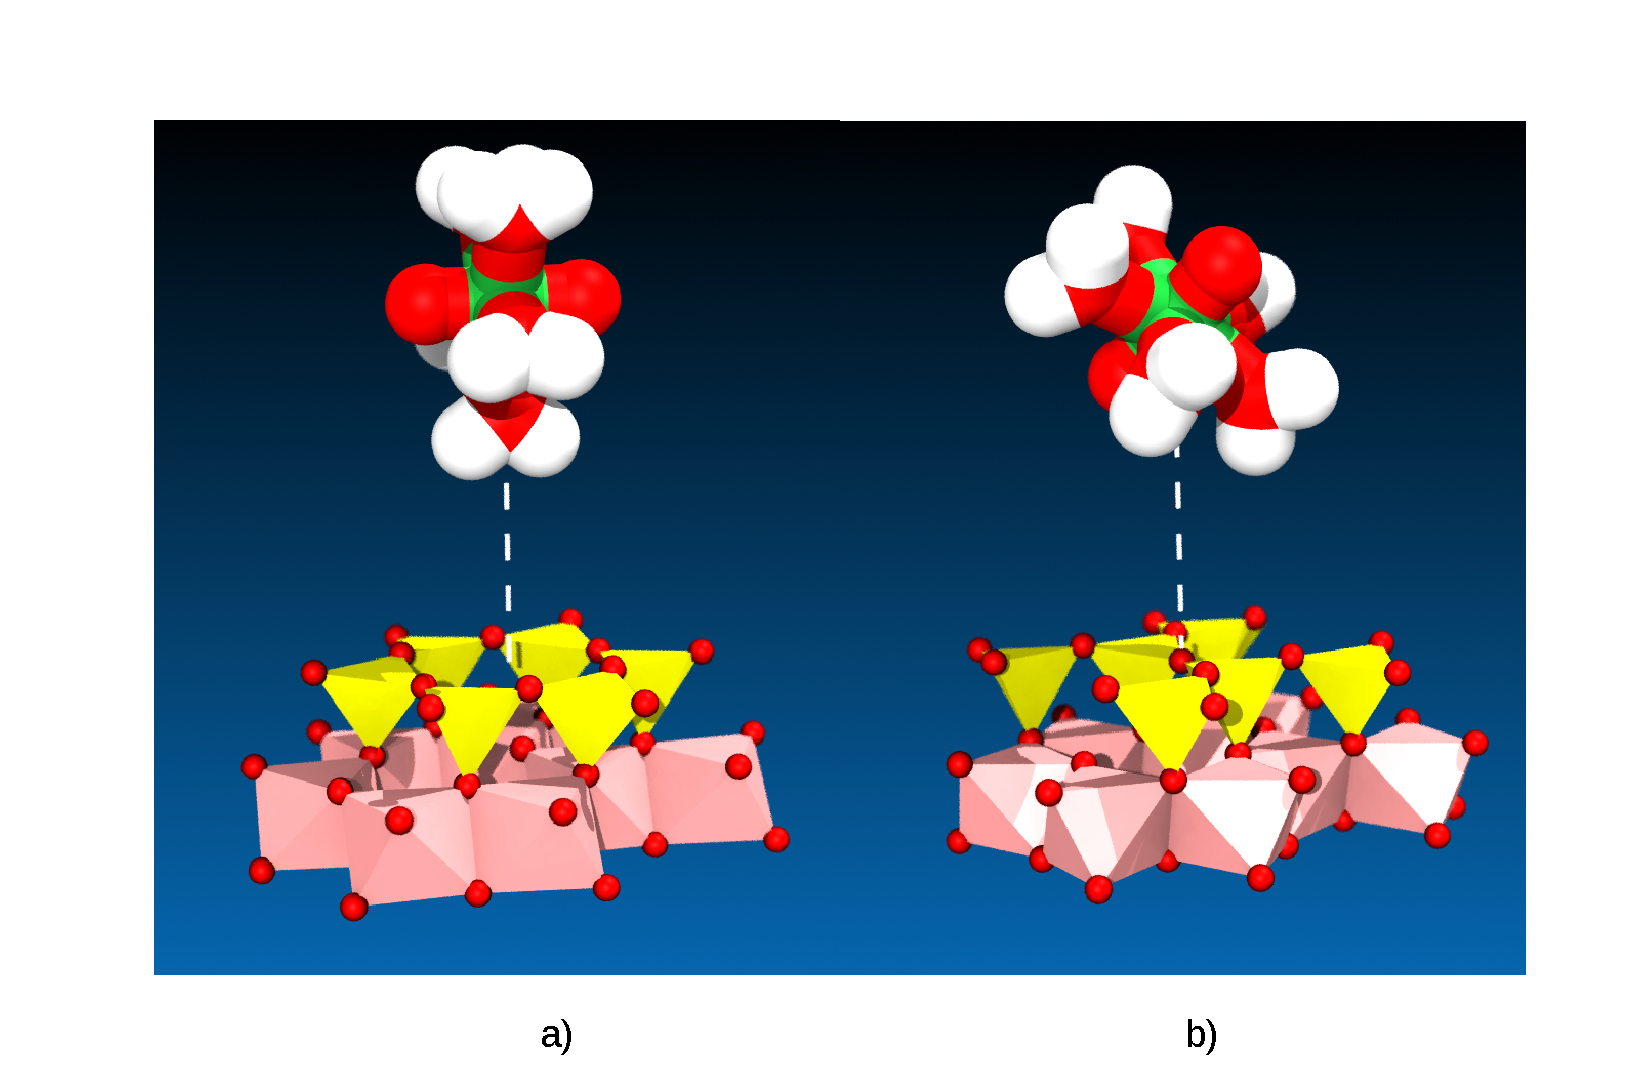
\includegraphics[width=10cm]{./images/scan.pdf}
\caption[QM scans used to parametrize the HIC]{Some of the clay cluster-hydrated ion scans 
used to parametrize the HIC 
potential. a) Hexagonal center scan with a uranyl axis tilt angle of 90º with respect to the 
surface normal. b) O-center cluster with a tilt angle of 45º. The color coding is as follows: Al 
octahedra (pink), Si tetrahedra (yellow), O atoms (red), uranium atoms (green), and H atoms (white)  
}
\label{scan}
\end{figure}

For the simulations of uranyl in montmorillonite clay interlayers the HI clay interaction (\gls{hic}) 
did not exist in the literature. A new strategy had to be developed since this was the first time 
the interaction of a HI with a surface was being studied. In the 
literature\cite{PhysChemChemPhys_Greathouse_2005,EnviSciTech_Greathouse_2006,JHazMat_Yang_2013,
JHazMat_Liu_2013,MolSim_Cygan_2014,
InorChemFronteirs_Zhang_2015,ClayMinSoc_Zaidan_2003,ClayMinSoc_Greathouse_2005} the 
Wipff-Guilbaud model of uranyl with combination rules was used, and therefore, to the best of 
our 
knowledge, this force field is the 
first \textit{ab initio} force field for actinyl-clay systems.


The force field was parametrized from 
the interaction energies of QM scans of \ce{[UO2*(H2O)5]^{2+}} approaching a
cluster of atoms carved from the clay surface (Figure \ref{scan}). The level of theory for the QM 
calculations was MP2 with 
RI\cite{RI1_Dunlap_JChemPhys_1979,RI2_JCompChem_Alsenoy_1988,RI3_Kendall_TheoChemAcc_1997,
RI4_Ahlrich_ChemPhysLett_1995,RI5_Ahlrich_TheoChemAcc_1997} and 
RIJCOSX\cite{RIJCOSX_ChemPhys_Nesse_2009} scaling reduction techniques due to the large size of the 
systems. U, Al and Si were described by Stuttgart semirelativistic pseudopotentials and their 
recommended 
basis sets\cite{U_ecpbasis,H-Rn_ECPbasis_PhysChemChemPhys_Ahlrichs_2005}; O and H were described by 
the 
aug-cc-PVDZ basis 
sets\cite{DunningBasisSet1_Dunning_JChemPhys_1989,DunningBasisSet2_Dunning_JChemPhys_1994,
DunningBasisSet3_Dunning_JChemPhys_1993,
DunningBasisSet4_Dunning_JChemPhys_1992,DunningBasisSet5_Dunning_JChemPhys_1996}. The interaction 
potential function had the following mathematical definition: 
 \begin{align} \label{eq_EHIC}
 E_\text{HIC}=& E_{\text{Coul.}}+E_{\text{non-Coul.}} \\ \nonumber
=&\sum_{i}^{\text{aqua ion}}\sum_{j}^{\text{clay}}\,\frac{q_iq_j}{r_{ij}}
+\sum_{i}^{\ce{U},\,\ce{O_{yl}},\,\ce{O_{I}}}\,\sum_{j}^{\ce{O_{clay}}}\,\frac{C_4^{ij}}{r^4_{ij}
} +
 \frac{C_6^{ij}}{r^6_{ij}}+\frac{C_8^{ij}}{r^8_{ij}}+\frac{C_{12}^{ij}}{r^{12}_{ij}} \nonumber
 \\&+\sum_{i}^{\ce{O_{yl}}}\,\sum_{j}^{\ce{Si}}\,\frac{C_4^{ij}}{r^4_{ij}}+
 \frac{C_6^{ij}}{r^6_{ij}}+\frac{C_8^{ij}}{r^8_{ij}}+\frac{C_{12}^{ij}}{r^{12}_{ij}} \nonumber
\end{align}
The root mean square error of the fit was $\sim$\SI{5}{\kcalmol}, a reasonable value
considering that the interaction energies can be as low as \SI{-100}{\kcalmol}. Structures 
obtained from the MD trajectories were used as a test set of data to check if the 
HIC potential reproduced the quantum interaction energies in structures outside of the 
training data set. 

 A good indicator of the quality of the force field is that it reproduces the experimental finding 
that the first-shell is identical in the clay as in aqueous 
solution.\cite{GeoCosmoAct_Catalano_2005} This outersphere complex 
formation was not imposed on the model. Therefore it was observed because the force field 
made this 
phenomenon to be favored over a partial dehydration into the tetrahydrate. In addition, the 
tilt-angle of the uranyl axis was compatible with the experimental evidence that showed it to be 
neither perpendicular nor parallel to the clay surface.\cite{MinWatIntClEq_Denecke_1999}

\section[Physico-chemical properties of actinyls in solution]{Physico-chemical properties of 
actinyls in solution}
MD simulations were run on the actinyl hydrated ions in aqueous solution with the 
newly developed HIM \textit{ab initio} force fields. In general, the properties calculated related 
closely to their experimental values. In addition the properties are of a 
wide variety: structure, dynamics, spectroscopy and thermodynamics. This good correlation
with experiment and the fact that the force field is \textit{ab initio} gives us  
confidence when computing properties that cannot be compared to experiment. 

The theoretical 
$\Delta H_\text{hyd}$ of the doubly-charged actinyls was fairly close to the value given by 
Marcus\cite{JChemSoc_Marcus_1986} for uranyl although further away from the value of 
Gibson\cite{JPhysChemA_Gibson_2005}. In the case of  \ce{[NpO2]^{+}}, the $\Delta 
H_\text{hyd}$ value matched the experimental value of 
Gibson\cite{JPhysChemA_Gibson_2005}. 
The translational self-diffusion coefficients of actinyls overestimated their experimental values. 
We found this to be caused by the overestimated diffusivity of water by the TIP4P bulk water 
model since the normalization of the coefficients by those of water 
gave a close agreement between theory and experiment. 

Our estimation of normal mode frequencies 
with respect to infrared and Raman spectra was satisfactory (maximum relative error of 15\%) 
considering 
that the B3LYP potential energy surface limits the model accuracy. If the NEVPT2 force field 
developed for \ce{[NpO2]^{+}} is used in simulation, the frequencies of the symmetric and 
asymmetric stretchings is even closer to experiment than if the DFT force field is used. This 
follows the 
idea that \textit{ab initio} force fields can be improved by improving the QM data set. 

Despite the 
specificity of $E_\text{IW1}$ and 
$E_\text{IMC}$, all hexavalent actinyls, 
\newline\ce{[AnO2*(H2O)5]^{2+}}, presented very similar physico-chemical properties: solvation 
structure, diffusion coefficients, hydration enthalpies ($\Delta H_\text{hyd}$), and second-shell 
mean 
residence times. The only exceptions were their vibrational and XAS spectra. 
Interestingly, 
even lowering the charge in the \ce{[NpO2]^{2+/+}} pair barely affected most hydration properties. 
The only exceptions were a small lengthening of the distances, a decrease of $\Delta 
H_\text{hyd}$ and shortening of the second shell mean residence times. Therefore, knowledge of a 
single actinyl in 
these regards can be generalized to the whole family. This is an interesting conclusion for 
experimentalists who can choose to work with the least radiotoxic of them, uranyl, when 
dealing with the properties that we find equivalent. 

An interesting outcome of the actinyl studies was understanding their hydration. Since the cation 
is a linear molecule, the asymmetry of the solvation required different analysis tools than for
conventional cations. Integrating the RDF of the second shell gave second-shell coordination 
numbers of 30, much higher than the other values in the literature, $\sim$20. The 
reason for such number is that the RDF assumes spherical symmetry and spherically averages the 
distribution. When 
facing with non-spherical problems, non-spherical techniques must be employed. Using the 
multisite cavity coordination number\cite{JChemTheoComp_ESM_2013} second-shell coordination 
numbers of 22-23 are obtained. The method gives similar results if used on other actinyl models. 
Angularly-resolved RDFs were also used to investigate the solvation structure. 



\begin{figure}
\centering 
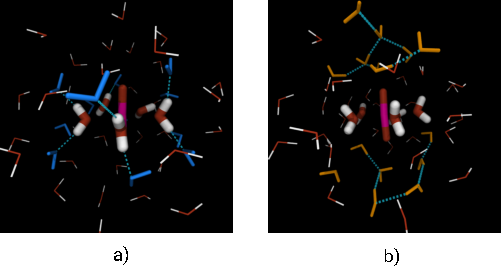
\includegraphics[width=10cm]{./images/An_VI_solvation.pdf}
\caption[Snapshots of \ce{[NpO2*(H2O)5]^{2+}} solvation]{MD snapshots of
\ce{[NpO2*(H2O)5]^{2+}} in water. a) Equatorial water molecules solvating the first-shell 
hydrophilically (blue). a) Axial water molecules hydrophobically solvating the \oyl 
atom (orange). }
\label{ActinylSolvation}
\end{figure}


No hydrogen bonding was found between water molecules and the \oyl atoms. This agrees with 
\textit{ab initio} MD 
simulations\cite{JACS_Buhl_2005,JChemPhys_Nichols_2008,JPhysChemA_Frick_2009} and classical 
simulations using 
\textit{ab initio} force 
fields\cite{JACS_Roos_2005,PhysChemChemPhys_Pomogaev_2013,JPhysChemB_Tiwari_2012}. We 
hypothesize that this apical hydrogen bond could be an artifact 
of empirical force fields\cite{JMolStr_Wipff_1996,JPhysChem_Wipff_1993,JPhysChemA_Kerisit_2013} and 
static QM calculations\cite{ChemPhys_Siboulet_2006}. We describe actinyls as anisotropic 
amphiphillic solutes which have a conventional solvation sphere caped at the poles by hydrophobic 
regions. 


Two clear solvation regions are observed. The equatorial region has the typical first-second 
shell
interactions of cations: the first-shell water mo\-le\-cu\-les form two hydrogen bonds with 
the 
second-shell ones, 
i. e. a 
hydrophilic solvation structure. Axially there is a hydrophobic solvation: the water 
mo\-le\-cu\-les 
form 
water-water structures around the \oyl atoms without interacting directionally with it. The final 
picture is that actinyls are amphiphillic anisotropically solvated solutes that have conventional 
cation solvation caped at the poles by hydrophobic regions (Figure \ref{ActinylSolvation}). This 
solvation is very unusual since a very small and highly charged cation holds two distinct
solvation regions.  

The most important achievement of this part of the thesis is the proposal of a general picture 
of the solvation of actinyls. Our view concurs with other works in the 
literature\cite{JACS_Roos_2005,PhysChemChemPhys_Pomogaev_2013,JPhysChemB_Tiwari_2012,JACS_Buhl_2005,
JChemPhys_Nichols_2008,JPhysChemA_Frick_2009}. Nevertheless, our picture stands on the extension of 
a robust methodology due to:
\begin{enumerate}
 \item The ability of the hydrated ion model 
to capture complicated 
many-body effects. 
 \item Our explicit parametrization of 
the bulk-HI interaction which separates our modeling from the rest of \textit{ab 
initio} force fields. Additionally, this interaction is universal among actinyls. 
\item The use of a classical potential allowed reaching larger 
system sizes and timescales than in \textit{ab initio} MD.
\end{enumerate}
\section[Modelling of actinyl EXAFS spectra]{Modelling of actinyl EXAFS 
spectra}\label{ModelXASSpectra}


The theoretical EXAFS spectra of the actinyls was calculated from the MD trajectories using the 
B3LYP level force fields. Here we shall not refer to americyl since its particular case will be 
explained in the next section. The simulated EXAFS spectrum of uranyl gave a reasonable agreement 
with the 
experimental one. Nevertheless, the rest of actinyls showed a qualitative agreement but far 
from that of 
uranyl or of other cations modeled using the group's methodologies. Since uranyl is the only closed 
shell actinyl of the set, we wondered if the potential energy surface used to build the force field 
was biased by the mean-field treatment done by unrestricted DFT in the open-shell systems. The 
NEVPT2 calculations of the actinyls had the effect of lengthening the An-\oyl distance and as a 
result a shortening of the An-\ofs distance. Although the changes are in the order of hundredths of 
an angstrom, these may cause a certain impact on the EXAFS spectra which are quite sensitive to 
structure. 

We calculated the theoretical EXAFS of \ce{[NpO2]^{+}} using the NEVPT2-level \textit{ab initio} 
force field. There was a significant improvement in the correspondence of the spectra with 
experiment with respect to the correspondence obtained using the DFT-level force field. The 
increase of the level of theory produced overall an improvement in the correspondence with 
experiment of the spectra. Nevertheless, the shoulder at low $k$ appears to be the most 
complex to predict since in this region of the spectrum both An-\oyl and An-\ofs have 
significant weight.

\section[Modelling of americyl XAS spectra]{Modelling of americyl XAS spectra}
Our modeling of americyl XAS spectra was an example of how theory and 
experiment can breed deep insights when combined. This part of the project started when trying 
to compare our theoretical americyl spectrum to experiment. We found that the only available 
experimental EXAFS spectrum were of a mixture of Am(VI)/Am(III), 
published in 2016.\cite{JRadioanNucChem_Riddle_2016} The experimentalists 
were unable to disentangle 
the mixture spectrum into the spectra of the two species. In addition, their modeling of the 
EXAFS equation gave some unusual structural parameters. They obtained a Debye-Waller factor for the 
Am-\oyl distance which was higher than for Am-\ofs. This is unusual since covalent bonds as the 
oxo-bond (\ce{Am=O}) 
are generally stiffer than coordinative bonds (Am-\ofs) and thus have lower thermal dispersion. 
With this information in mind we decided to tackle the problem with some of our newly developed 
actinyl force fields.

\begin{figure}
\centering 
\includegraphics[width=0.7\columnwidth]{./images/Exafs.png}
\caption[EXAFS spectra of Am]{L$_\text{3}$-edge $k^2$-weighted EXAFS spectrum of Am 
experimental (dashed) and simulated 
(solid). Top: $Am^{3+}$ aqueous solution experimental\cite{EnvSciTech_Stumpf_2006} and simulated 
spectra. Middle: pure \ce{[AmO2]^{2+}} simulated spectrum (red) and of the ionic 
mixture\cite{JRadioanNucChem_Riddle_2016}. Bottom: Experimental spectrum of the ionic 
mixture\cite{JRadioanNucChem_Riddle_2016} and simulated spectrum of \ce{[AmO2]^{2+}} and 
\ce{Am^{3+}} weighted with  70/30 (pink) and 55/45 (blue) ratios.}
\label{XAS_Am}
\end{figure}

MD simulations of aqueous \ce{[AmO2*(H2O)5]^{2+}} and 
\ce{[Am*(H2O)8]^{3+}} were run  using the newly developed force fields; \textit{ab initio} for 
Am(VI) and empirical for Am(III). The theoretical EXAFS and XANES spectra for both compounds were 
calculated. The Am(III) spectra matched the experiment as expected since the potential was built 
\textit{ad hoc} to do so. We 
generated the weighted sum of the XAS spectra of both pure 
theoretical spectra to produce the theoretical spectrum of the mixture. The weights were given 
according to the relative abundance of the species reported by the experimentalists. The agreement 
of the theoretical spectrum of the mixture and experiment was really good. The 
experimentalists determined that the initial Am(VI)/Am(III) ratio of the species, 70/30, was 
likely 
to have changed 
due to radiation damage or the redox instability Am(VI). Varying the weights of the simulated 
spectra of Am(VI)/Am(III) we found a 55/45 ratio to give the best match between the experimental 
and theoretical spectra (Figure \ref{XAS_Am}). 

In this work we simulated XAS spectra (EXAFS and XANES) of a 
mixture of species which is consistent with the experiment. This is a very stimulating 
result given the complexity of EXAFS modeling in general, specially on actinyls (see 
Chapter \ref{art3.5}) and in a mixture of species. The results provide confidence in the 
developed methodology.

This synergic theoretical-experimental findings gave strong evidence that our simulation of 
\ce{[AmO2*(H2O)5]^{2+}} was fairly accurate. This allowed us to predict the distances,
Debye-Waller factors and XAS spectra of pure americyl aqueous solution, which has never been 
obtained experimentally. In addition, our parameters recover the usual trend that the stronger 
bond 
should 
have the 
lowest Debye-Waller factor.

\section[Diffusion of uranyl in montmorillonite clay]{Diffusion of uranyl in montmorillonite 
clay}

MD simulations were run on hydrated montmorillonite clay introducing uranyl cations 
in the interlayer in exchange for the \ce{Na+} cations. We studied the diffusion and dynamics of 
the uranyl cations inside the interlayers. Two simulations were run. One contained a single 
uranyl cation 
per interlayer and the other one four ions per interlayer. 
We have studied only uranyl 
but given the similarities between the actinyls, the information is likely to be extended to 
the rest of them. This is particularly important since the most hazardous actinoids of spent 
nuclear 
fuel are neptunium,plutonium and americium.

\begin{figure}
\centering 
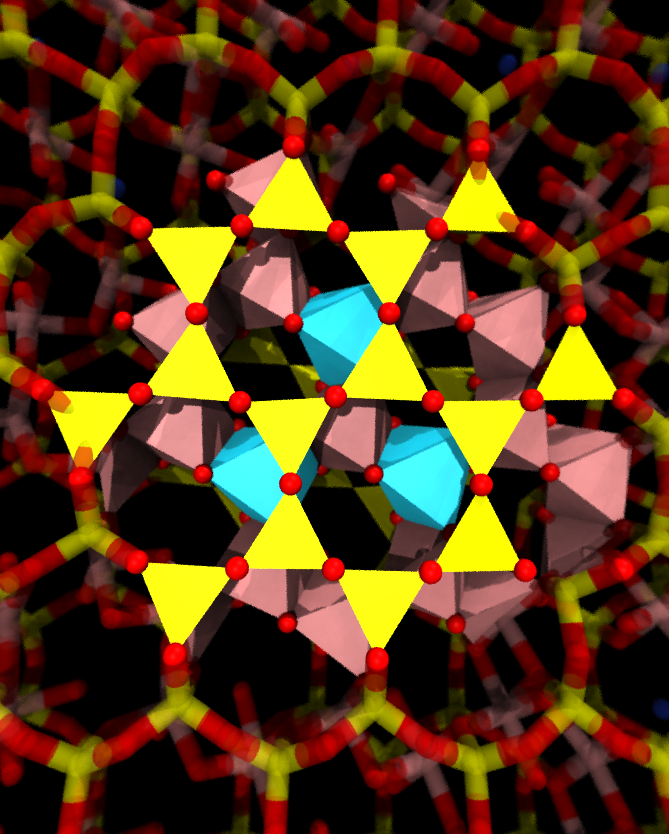
\includegraphics[width=5cm]{./images/site.png}
\caption[Strong interaction site for uranyl]{Interaction site for uranyl at the 
montmorillonite clay surface: three Mg octahedra 
separated from each other by a single central Al octahedron. Al 
octahedra (pink), Mg octahedra (blue), Si tetrahedra (yellow), O atoms (red), uranium atoms 
(green), and H atoms (white) 
}
\label{site}
\end{figure}

The diffusion of the uranyl cations within the clays was greatly hindered with respect to solution. 
The diffusion occurs 
on the clay surface with very few transitions of the cations from one surface to the middle of the 
interlayer or the other surface. This work is the first to calculate from MD the 
constrictivity factor,
$\delta_{int}$, which measures the uranyl diffusivity in the interlayer with respect to 
solution. Our estimation of $\delta_{int}$ was close to one order of magnitude higher than 
experiment\cite{TaiMine_Moore_2011} encouraging the idea that on broad strokes 
we capture the physics of the system. The disagreement between theory and experiment should be put 
in context with the difficulties of modeling a very homogeneous system like real clays in 
complex electrolytes. The main causes of  discrepancy could be the 
relatively short-time of the simulation, the inaccuracies in force field development, the 
differences between our idealized system and the real clays, and the fact that the $\delta_{int}$ 
is a fitted parameter in Fick-equation modeling and other effects could contribute. 

The key finding of the work was the identification of strong interaction sites for uranyl. We 
observed that 
uranyls tightly bound to the surface in regions were three 
substitutions occurred forming a triangle of Mg-octahedra around an Al-octahedron (See 
Figure \ref{site}). The electrostatic potential maps of 
the surface showed that the strong interaction is driven by electrostatics. The identification 
of the sites allowed us to propose a hopping diffusion me\-cha\-nism. In this mechanism the 
uranyl 
cations oscillate around the interaction sites until they are able to escape and diffuse away 
until reaching another site, then the motion becomes oscillatory again. 

The other interesting result of the simulations was that increasing the concentration of 
uranyl cations in the clay increased their diffusion. We found the explanation for this 
phenomenon in the strong interaction sites. If there are more uranyl cations in the interlayer 
there will be more occupied sites on average and thus a diffusing cation will have larger 
displacements before falling into a site. In addition, the repulsion between cations can promote 
one cation ``pushing'' others out of their sites also increasing diffusion. 

The microscopical information obtained from our studies 
gives a complementary view to uranyl diffusion in clays to what is typically studied with 
macroscopic Fick-equation modeling.

\section[Development of a local hydrophobicity/hydrophilicity fingerprint]{Development of a 
local hydrophobicity/hydrophilicity fingerprint for enhanced 
sampling 
simulation}

A local fingerprint for hydrophobicity and hydrophilicity was developed inspired by the 
expansion 
of entropy in terms of increasing correlation terms (Equation \ref{expansion}). The fingerprint 
for solute heavy atom, $i$, in aqueous solution is:
\begin{equation}
S_{\text{s}}^{i}=-2\pi \rho_{\text{w,loc}} \int_{0}^{\infty}\left\{\right. g_{i\text{w}
}(r)\ln\left[g_{i\text{w}}(r)\right] 
-g_{i\text{w}} (r)+1\left.\right\}r^2dr
\label{sij}
\end{equation}
Where $\rho_{\text{w,loc}}$ is the local water density around the solute atom and $g_{i\text{w}
}(r)$ is the radial distribution function (\gls{rdf}) of atom $i$ with water molecules, w. 
$S_{\text{s}}^{i}$ is 
then rescaled into  $h_i$, which is defined to be 1 for water and -1 for 
methane to give perspective to the fingerprint numerical values. The reader must be cautioned that 
the fingerprint is not a measurement of hydration entropy, since it is only one term of the 
expansion of the translational entropy of the system. Our goal is to find a fingerprint that 
measures in simple fashion hydrophobicity or hydrophilicity locally. 



\begin{figure}
\centering
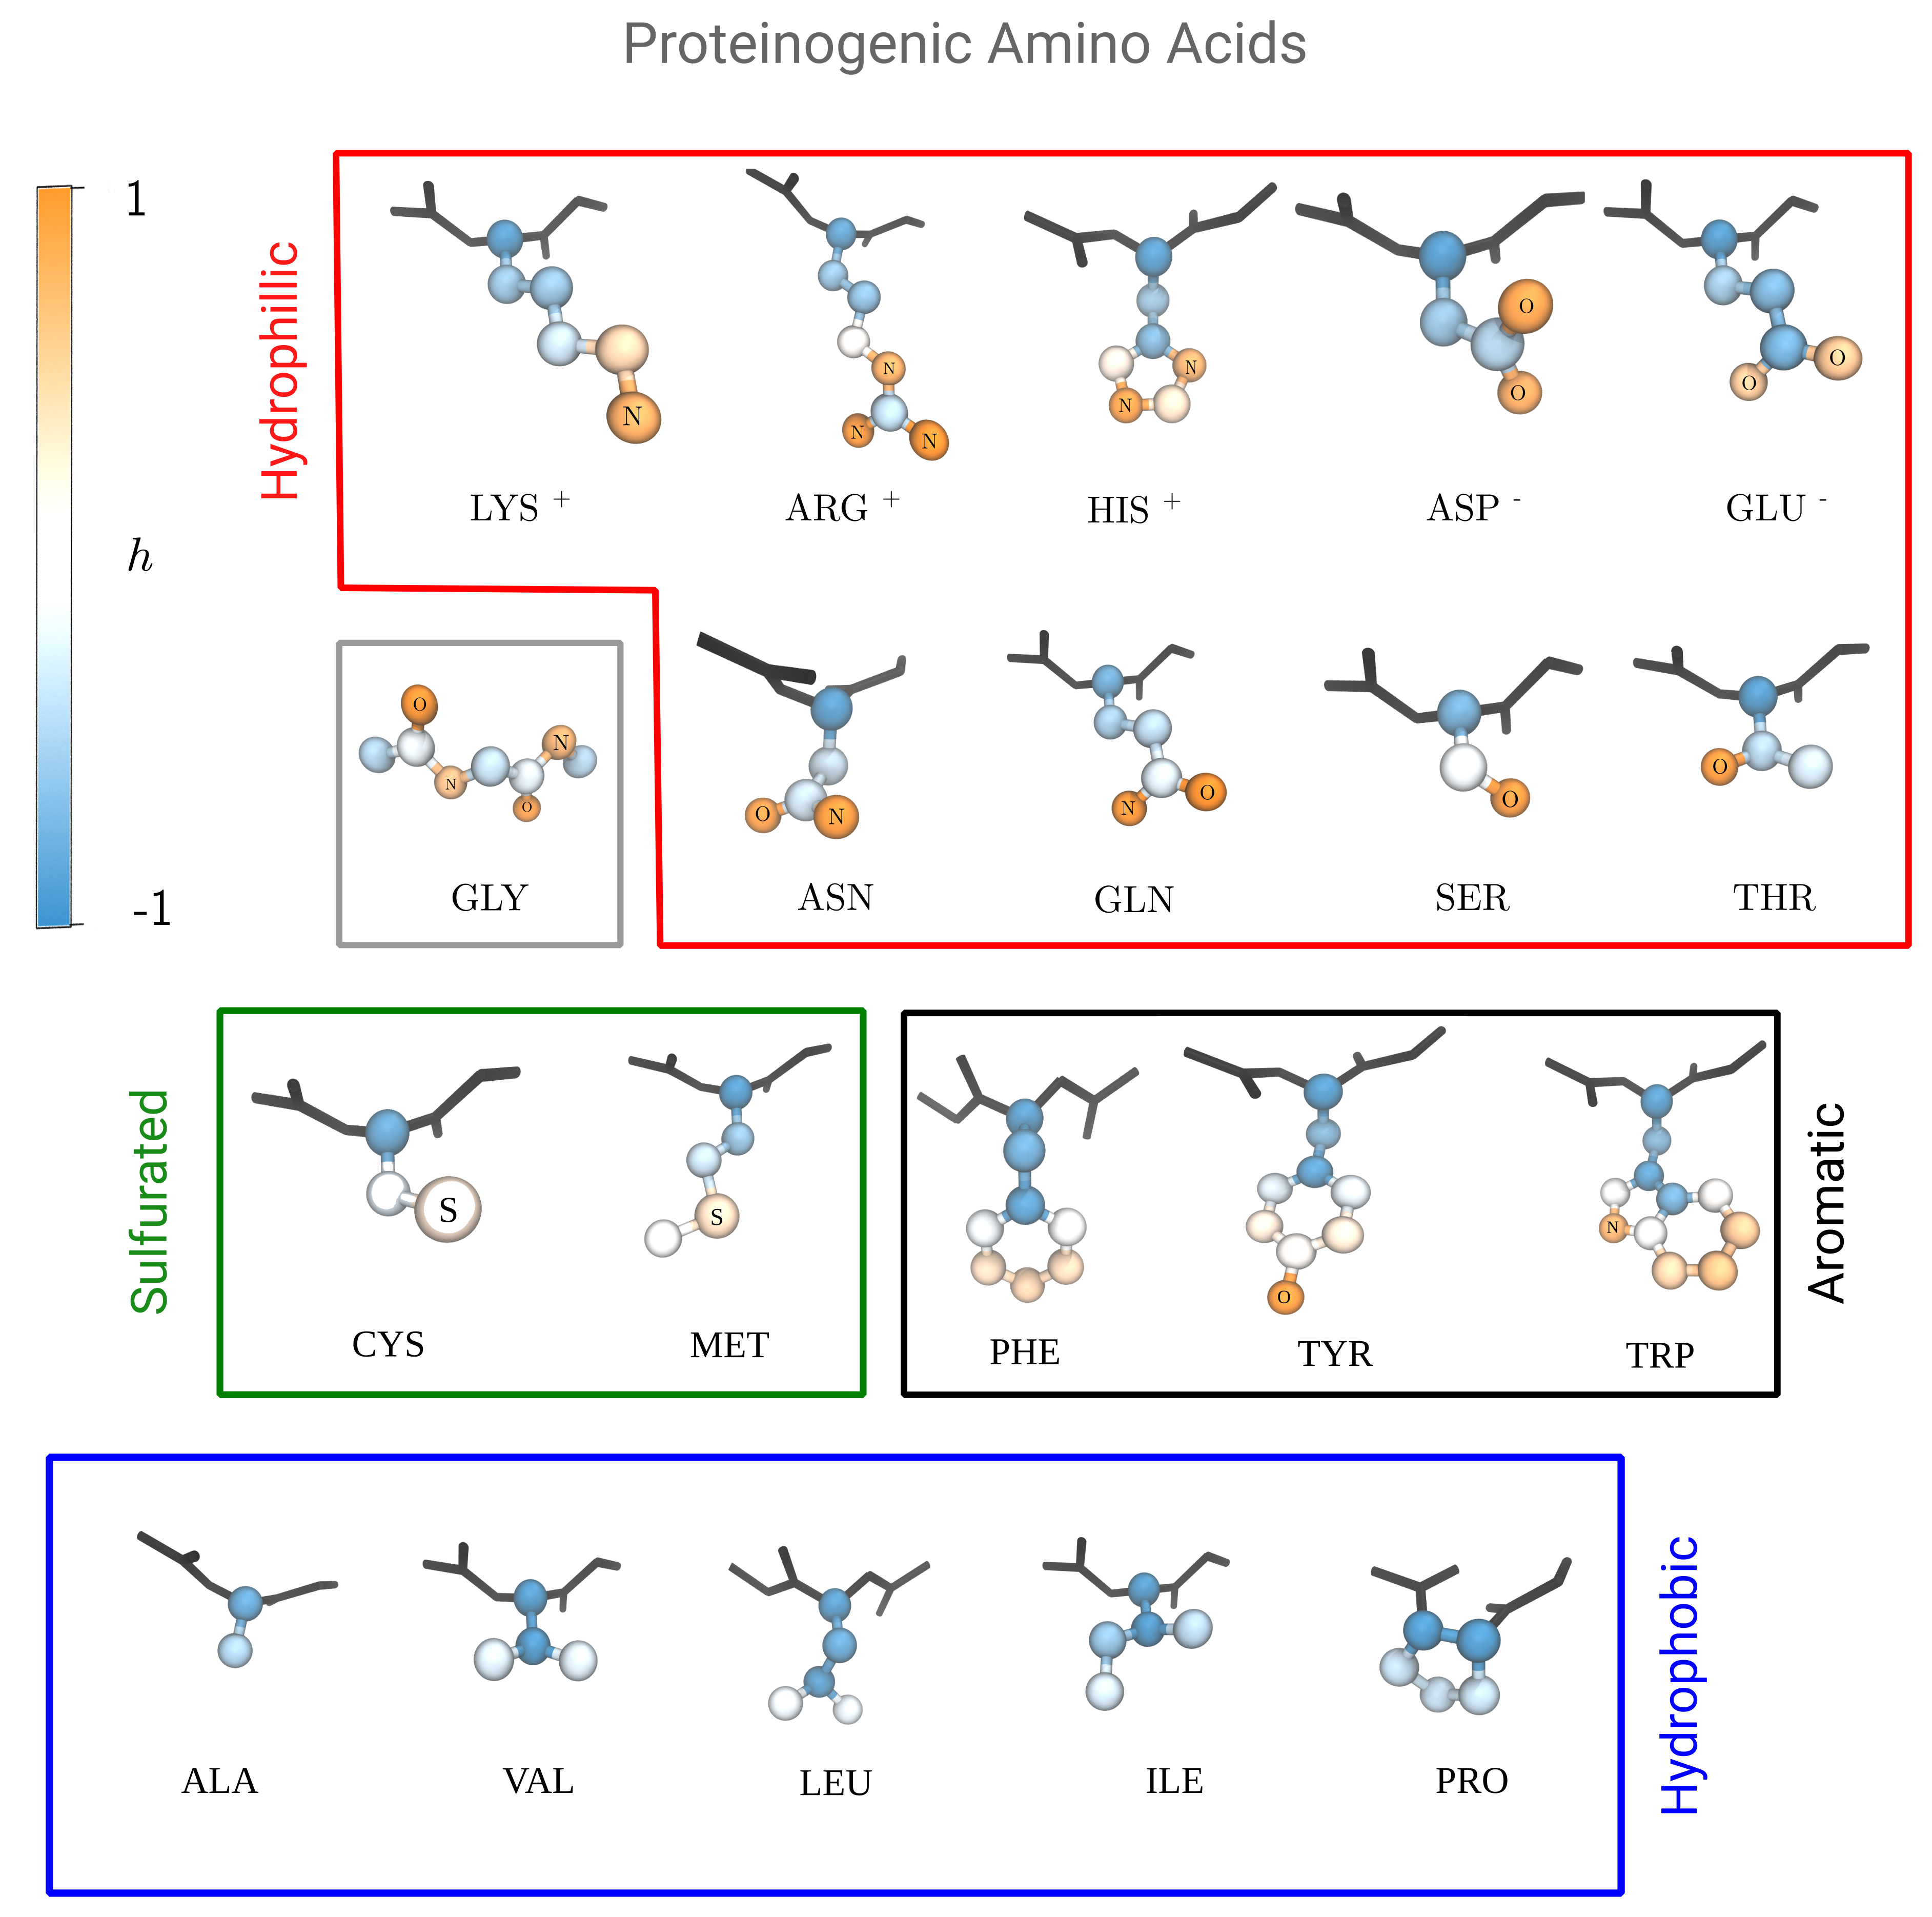
\includegraphics[width=\columnwidth]{./images/aa.png}
\caption[Fingerprint values for the 20 aminoacids]{ Structure of the 20 proteinogenic amino 
acids with their heavy atoms colored by their 
hydrophobicity/hydrophilicity fingerprint values. The color scale varies from hydrophilic 
(orange),
to intermediate (white), to hydrophobic (blue). Hydrogen atoms are omitted. Unlabeled atoms are 
carbon atoms. The backbone is only shown for glycine since its fingerprint value is very similar in 
all cases. }
\label{aa}

\end{figure}
The fingerprint was able to correctly classify as hydrophilic or hydrophobic the atoms of the 
20 
proteinogenic amino acids which have a large variety of chemical groups and  environments. 
Figure \ref{aa} shows the amino acids with their heavy atoms colored 
according to their $h$ values. It is striking that some of 
the aromatic atoms are colored as 
slightly hydrophilic. Interestingly this can be explained because experimentally the 
properties of 
aromatic compounds are not as hydrophobic as aliphatic 
carbons\cite{JPhysChem_McAuliffe_1966,JSolvChem_Cabani_1981,Ben-Amotz2016,Harris2016}. 

The fingerprint is very 
simple in formulation and calculation. It just takes as input the RDF which is routinely 
obtained in simulation. It is a local fingerprint 
that measures atomic hydrophobicity/hydrophilicity in contrast with most scales in the 
literature which focus on the whole residue\cite{Simm2016}. The maximum fingerprint value of 
the amino acid was found to correlate with its hydration free energy. The correlation is not 
very strong but is very similar to the one obtained by Schauperl et al\cite{Schauperl2016}. In 
their 
work they used a much more complex and computationally demanding technique that unlike our 
fingerprint is dedicated fully to thermodynamical property calculation. Therefore, our 
fingerprint gives a measurement of the hydrophobicity or hydrophilicity which is simple, 
local, inexpensive and useful to classify the atoms of molecular solutes. 

The instantaneous value of the fingerprint can be calculated on-the-fly in MD
simulation. The fingerprint can become a CV in enhanced sampling simulations using a 
differentiable continuous version of the RDF. The fingerprint serves as a 
desolvation CV. In order to prove the usefulness of the fingerprint as a 
CV, we ran WTMetaD simulations. The model system chosen was a host-guest system in 
aqueous solution. Host-guest systems are model systems for protein-ligand complexes. The 
host is a barrel-shaped molecule that can host a smaller molecule, the guest. In this system 
in 
particular the literature showed that desolvation of the host was a crucial slow mode of 
the binding\cite{Bhakat2017a}. Therefore, in addition to a binding CV (a contact map) a 
desolvation CV (the fingerprint CV) had to be used in order to converge the simulations.

Using the 
fingerprint as a desolvation CV allowed the convergence of the WTMetaD simulations. 
This was done in a single simulation whereas in the literature it required an 
additional free energy perturbation calculation\cite{Bhakat2017a}. The analysis of the free 
energy surface of the host-guest binding showed that the removal of the two last water 
molecules within the barrel is a kinetic barrier in the process. 

The fingerprint serves as 
an alternative to other solvation CVs like the coordination number of water molecules which just 
counts the number of water molecules around a solute atom. Our CV is more detailed since apart from 
measuring the amount of solvation around the molecule it also accounts for the structure 
of this solvation.

\subsection[Application to actinyl hydration]{Application to actinyl hydration}

 The fingerprint of the actinyl pentahydrate atoms was calculated. The fingerprint has mixed 
results in classifying the atoms of the actinyl pentahydrates and appears to be too coarse for 
such systems. The fingerprint mistakenly classifies the actinoid atom as hydrophobic. This had 
also been observed in \ce{Na+}. It also mislabels the \oyl atom as hydrophilic. We attribute 
this fact to the use of the total RDF which captures the water molecules of the 
bridge-solvation region that do not directly solvate the \oyl atom. Using an angle-solved RDF 
in the fingerprint correctly classifies both oxygen atom types but unfortunately considers the 
\ofs atom less 
hydrophilic than bulk water. 

A future improved fingerprint should probably make use of orientational pair entropy in 
addition to some technique to consider the anisotropicity of the solute in complex 
environments.


\bibliographystyle{achemso}
\bibliography{./library,./extrabib}
